\section{GA-P}

GA-P se trata de una mejora de Programación Genética. Esta propuesta fue publicada en 1995 por investigadores de la Universidad de Georgia \cite{primerGAP}.

Esta modificación está pensada especialmente para problemas donde Programación Genética se utiliza para regresión simbólica.

\subsection{Como funciona GA-P}

Uno de los principales problemas de Programación Genética es el aprendizaje de las constantes numéricas. GA-P soluciona este problema siendo un híbrido entre Programación Genética y Algoritmo Genético.

GA-P, además de utilizar la representación en árbol de Programación Genética, añadirá un cromosoma de forma que las constantes numéricas en el árbol se referirán a posiciones en dicho cromosoma. De esta forma GA-P, además de ajustar el árbol, también ajustará el cromosoma como si fuera un problema de Programación Genética para así buscar unos mejores valores de las constantes numéricas sin tener que realizar operaciones con estas para obtener cierto valor.

\begin{figure}[H]
    \centering
	  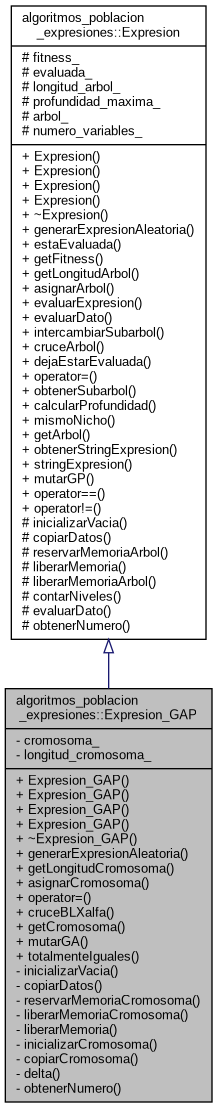
\includegraphics[width=0.6\textwidth]{expresion_gap.png}
    \caption{Ejemplo de una expresión de GA-P con un cromosoma asociado.}
	 \label{fig:expresion_gap}
\end{figure}

De esta forma, como vemos en la figura \ref{fig:expresion_gap}, los nodos de las expresiones tendrán asociados variables del problema (como $x$ en el ejemplo), o constantes, las cuales tendrá un valor asociado en el cromosoma de la expresión. Por ejemplo, con los valores actuales de la imagen la expresión sería la siguiente:

$$ -6 \cdot ( (-3.9 / x) + 12 ) $$

Esta representación nos permitirá entrenar la parte de Programación Genética del modelo con los operadores vistos en Programación Genética, y por otra parte ajustar las constantes numéricas utilizando el cromosoma, la parte de Algoritmo Genético.

\subsection{Operadores de GA-P}

Además de los operadores de la parte de Programación Genética, que se mantendrán, GA-P utilizará operadores para la parte de Algoritmo Genético. En este caso se podrían aplicar todo tipo de operadores de codificación real ya que existe una gran variedad, pero se comentarán los operadores más comunes y que utilizaremos en este caso.

\subsubsection{Operador de cruce}

Como operador de cruce utilizaremos el cruce BLX-$\alpha$, propuesto en 1993 por Larry J. Eshelman y J. David Schaffer \cite{cruceBLXalfa}.

Este operador de cruce se trata de una modificación del operador de cruce para cromosomas de codificación real de Radcliffe \cite{cruceRadcliffe}, en el que para cada punto de ambos cromosomas se escogía un valor aleatorio escogido de forma uniforme entre ambos valores reales.

BLX-$\alpha$ además de tomar en cuenta el intervalo entre ambos números de ambos cromosomas $I$, amplía dicho intervalo en un $\alpha \cdot I$, es decir, si al cruzar dos cromosomas, si el valor del padre es $x$ y el de la madre es $y$, $I = y - x$, utilizando el operador de cruce de Radcliffe el nuevo valor estaría en el intervalo $[x, y]$, mientras que utilizando el cruce BLX-$\alpha$ utilizará como intervalo $[x - I \cdot \alpha, y + I \cdot \alpha]$. Como vemos, BLX-$0.0$ sería equivalente al operador de cruce de Radcliffe.

Con esta modificación conseguimos que el operador de cruce sea capaz de tener una mayor exploración del espacio de búsqueda, además de evitar que los cromosomas converjan demasiado rápido.

\begin{figure}[H]
	 \centering
	 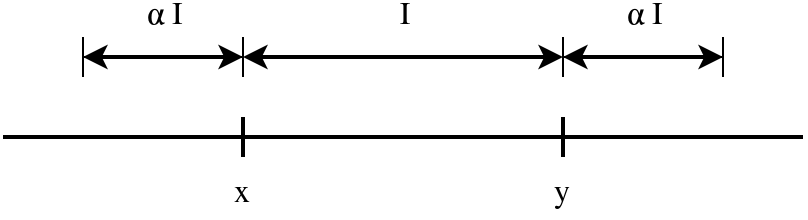
\includegraphics[width=0.6\textwidth]{blxalfa.png}
	 \caption{Ejemplo de un intervalo entre $x$ e $y$ al que aplicar BLX-$\alpha$.}
	\label{fig:cruceBLXa}
\end{figure}


\subsubsection{Operador de mutación}



\subsection{Problemas de GA-P}

\subsection{Modificaciones de GA-P}
